\documentclass{beamer}
\usepackage{HECbeamer}
% \usepackage{pgfpages}
% \pgfpagesuselayout{4 on 1}[letterpaper, landscape, border shrink=5mm]
\title[\color{white}{MATH 60604A \S~6f - Prediction from linear mixed models}]{\texorpdfstring{MATH 60604A \\Statistical modelling \\ \S~6f - Prediction from linear mixed models}{MATH 60604A \\Statistical modelling \\ \S~6f - Prediction from linear mixed models}}
\author{}
\institute{HEC Montréal\\
Department of Decision Sciences}
\date{} 

\begin{document}
\frame{\titlepage}
\begin{frame}
\frametitle{Prediction}
\bi
\item The random effects $\bs{b}$, are \alert{random variables} and not parameters (parameters are fixed,  but unknown quantities). 
\item We can always get \alert{predictions} for these random variables. 
\item Once we have predicted values for the $\bs{b}$ terms and estimates for the fixed effect parameters, $\bs{\beta}$, we can predict the outcome variables $\bs{Y}$ by its conditional mean. 
\ei
\end{frame}


\begin{frame}
\frametitle{Prediction: model \textbf{without} random effects}
\bi
\item \alert{If there are no random effects in the model} (for example, if we had fitted a model that directly specified the covariance structure using \code{repeated}), then we make predictions in the same way as we did for ordinary linear regression. 
\item That is, the prediction for $Y_{ij}$ is
\begin{align*}
\hat{Y}_{ij}=\hat{\beta}_0 + \hat{\beta}_1\mathrm{X}_{ij1} + \ldots + \hat{\beta}_p\mathrm{X}_{ijp}.
\end{align*}
\item This quantity is also the estimate of the \alert{mean} (at the \alert{population level}) of the response variable.
\ei
\end{frame}

\begin{frame}
\frametitle{Prediction: model \textbf{with} random effect}
\bi
\item If there are random effects in the model, the estimation of the \alert{marginal mean} (at the \alert{population level}) of the response variable for an individual with the characteristics of individual $j$ from group $i$ is
\begin{align*}
\hat{Y}_{ij}=\hat{\beta}_0 + \hat{\beta}_1\mathrm{X}_{ij1} + \ldots + \hat{\beta}_p\mathrm{X}_{ijp}.
\end{align*}


\item But we can also get predictions of the
values of the response variable for individual $j$ in group $i$
\item For example, in a model with a random intercept for group $i$, $b_{i}$,
 \begin{align*}
\hat{Y}_{ij}=\hat{\beta}_0 +\hat{b}_{i} + \hat{\beta}_1\mathrm{X}_{ij1} + \ldots + \hat{\beta}_p\mathrm{X}_{ijp}. 
\end{align*}

\item If, however, we want to get predictions for a \alert{new}
individual that was not included in the original dataset, then we have no choice but to use the mean prediction, because the random effect estimate of this group is not available.
\ei
\end{frame}

\begin{frame}[fragile]
\frametitle{Predictions for random effects}
\begin{tcolorbox}[colback=white, colframe=hecblue, title=\SASlang{} code for the random intercept model]
\begin{small}
\begin{verbatim}
proc mixed data=statmod.motivation;
class idunit;
model motiv = sex yrserv agemanager nunit / solution;
random intercept / subject=idunit type=vc solution;
ods output Mixed.SolutionR=re;
run;
\end{verbatim}
\end{small}
\end{tcolorbox}
\begin{small} The option \code{solution} in the command \code{random} is used to get predictions of the random effects. The command \code{ods output}
saves these in order to make diagnostic plots for the random effects.\end{small}
\end{frame}

\begin{frame}
\frametitle{Predictions of the random effects}
\begin{center}
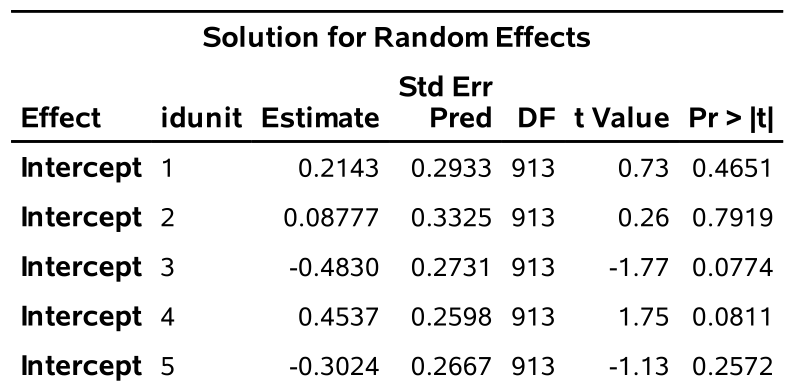
\includegraphics[width = 0.7\linewidth]{img/c6/slides7-e19}
\begin{align*}
 \vdots
\end{align*}
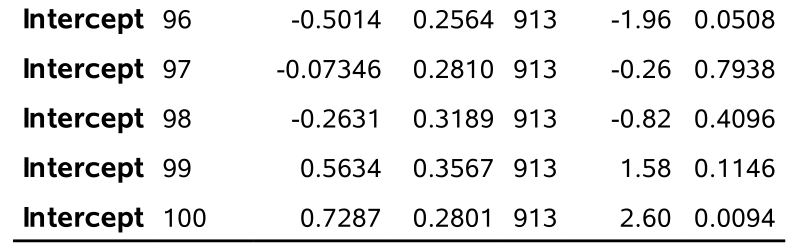
\includegraphics[width = 0.7\linewidth]{img/c6/slides7-e20}
\end{center}
\end{frame}

% \begin{frame}
% \frametitle{Predictions for the random effect terms of the first three units} 
% 
% \begin{center}
% \includegraphics[scale=0.5]{Figures/long118.pdf}
% \end{center}
% \begin{small} Only part of the table is shown here: the full table includes predictions for all $100$ units in the dataset. \end{small}
% \end{frame}
% 
\begin{frame}
\frametitle{Histogram of random effects}
We can plot histograms and quantile-quantile plots of the predicted random intercepts.
\begin{center}
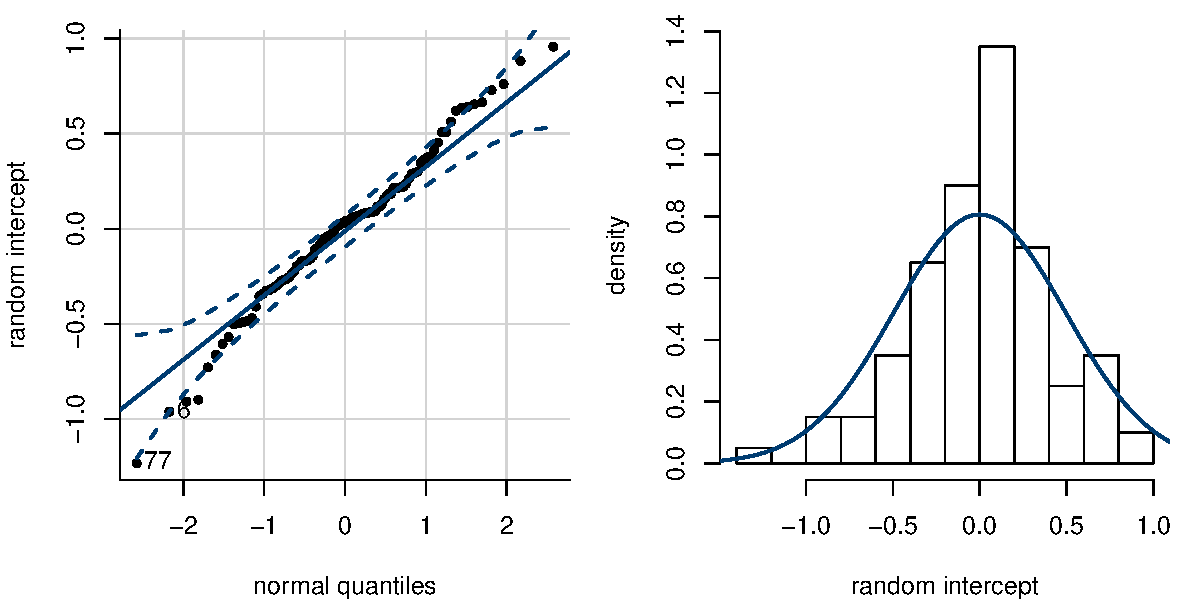
\includegraphics[width = 0.8 \linewidth]{img/c6/07-mixed-diagran.pdf}
% \includegraphics[width = 0.45 \linewidth]{Figures/long120.pdf}
\end{center}
These can help us check the normality assumption of the random effects (think of these as further residual diagnostics). Note that (by construction), the average of these random effects is always zero.
\end{frame}

% \begin{frame}
% \frametitle{Scatterplot of the random intercept $b_i$ as a function of $b_{1i}$}
% 
% \begin{center}
% \includegraphics[scale=0.35]{Figures/long121.pdf}
% \end{center}
% \bi
% \item We assumed that the two effects are independent. 
% \item This assumption can be relaxed in \code{proc mixed} by setting, e.g., \code{type = un}.
% \ei
% \end{frame}

\begin{frame}[fragile]
\frametitle{Predictions for observations $Y$}
\bi
\item With \code{\code{proc mixed}}, we can save the values \alert{for all observations in the data file}:
\bi
\item Predictions for the mean of the population (fixed effects),
\item Individual predictions (fixed and random effects).
\ei
\item This is done using the options \code{outpm}
and \code{outp}, respectively, in the \code{model} command.
\item \textbf{Trick}: in \SASlang{}, if you want predictions for new individuals, you can just include these in the data file with a missing response (with ``.''). These individuals will not be used in the estimation of the model
\ei
\end{frame}

\begin{frame}[fragile]
\frametitle{Prediction for new employees}
We assume that we want to get predictions for two new employees, one of whom is part of a unit already present in the dataset (\code{idunit=1}) and one that is part of a unit not in the original dataset (\code{idunit=101}). 


\begin{tcolorbox}[colback=white, colframe=hecblue, title=\SASlang{} code to input two new observations]
\begin{small}
\begin{verbatim}
data newdata; 
input nunit idunit idemployee yrserv sex 
     motiv agemanager; 
cards; 
9 1 10 5 0 . 40 
9 101 1 5 0 . 40; 
run; 

/* Merge observations with database */
data motivation; 
set statmod.motivation newdata; 
run;
\end{verbatim}
\end{small}
\end{tcolorbox}
\end{frame}

\begin{frame}[fragile]
\frametitle{Code to fit the model and get predictions}
\begin{tcolorbox}[colback=white, colframe=hecblue, title=\SASlang{} code to output predictions from a mixed model]
\begin{verbatim}
proc mixed data=motivation; 
class idunit; 
model motiv = sex yrserv agemanager nunit 
     / solution outp=prediction outpm=mean; 
random intercept / subject=idunit type=vc; 
run;
\end{verbatim}
\end{tcolorbox}
\bi
\item The data file used is \texttt{data=motivation}, which contains the $1018$ observations, but only the $1016$ observations from the original file are used in fitting the model. 
\item However, predictions will be made for all $1018$ observations in the files \texttt{mean} and \texttt{prediction}.
\ei
\end{frame}

\begin{frame}[fragile]
\frametitle{Population mean of the two new subject}
Output in file \code{mean}:
\begin{center}
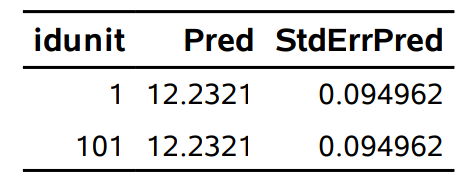
\includegraphics[width = 0.4\linewidth]{img/c6/slides7-e21}
\end{center}
\bi
\item The fitted mean ($12.23$) is the same in both cases because only the fixed effects were used and the two employees have the same values for the explanatory variables.
\ei
\end{frame}

\begin{frame}[fragile]
\frametitle{Predictions for the two new subjects}

Output in file \texttt{prediction}:
\begin{center}
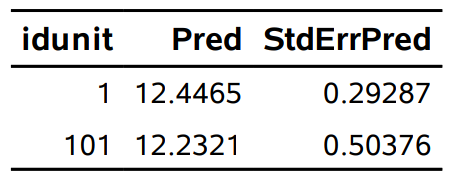
\includegraphics[width = 0.4\linewidth]{img/c6/slides7-e22}
\end{center}
\bi
\item This time, the random effects are used if they're available. Since unit $1$ was present in the model fitting, its random effect is used in making the prediction ($12.45$). 
\item However, the unit
$101$ was absent when fitting the model. Therefore, the prediction for the employee in unit $101$ is only based on the fixed effects in the model, 
meaning that we get the same predicted value ($12.23$) as before.
\item The standard errors for the individual predictions are larger, reflecting the added individual uncertainty arising from the errors and the random effects.
\ei
\end{frame}


\end{document}
